\chapter{Interfaccia di calibrazione}\label{ch:interfaccia}
Questo capitolo è incentrato sulle motivazioni, lo sviluppo e la realizzazione di una dashboard web per la calibrazione multipla di centraline AirQino.

% Motivazioni
\section{Motivazioni}\label{sec:motivazioni}
I sensori possono essere soggetti a molteplici processi di calibrazioni durante loro ciclo di vita (vedi \ref{sec:calib-intro}). Lo scopo è quello di trovare i coefficienti della curva che meglio approssima la relazione tra il segnale del sensore e un segnale di riferimento, da cui poter ricavare il valore calibrato a partire dal dato grezzo.

Attualmente, per tutte le centraline e sensori AirQino, il dato calibrato viene ottenuto con la seguente formula:

$$y(t)=k_{1} x(t)+k_{2} x^{2}(t)+k_{3} T_{int}(t)+k_{4}$$\smallskip

\clearpage

dove:

\begin{itemize}
  \item $x$ è il \textbf{dato grezzo};
  \item $k1...k4$ sono i \textbf{coefficienti di calibrazione} ottenuti applicando un modello di regressione ai valori misurati rispetto ad un segnale di riferimento;
  \item $T_int$ è la \textbf{temperatura interna} della centralina al tempo $t$;
  \item $y$ è il \textbf{valore calibrato}.
\end{itemize}

I coefficienti $k1...k4$ sono memorizzati nella tabella \textit{field\_calibration} del database AirQino. Si ha
un set di coefficienti per ogni terna centralina, sessione, sensore: in questo modo si possono utilizzare parametri di calibrazione diversi per \textit{sessioni} diverse. I dati possono essere inseriti attraverso un form accessibile dalle pagine di amministrazione.\\

Questa soluzione risulta però poco flessibile, in quanto ogni singolo coefficiente di ogni sessione e di ogni centralina deve essere inserito manualmente. Come soluzione a questo problema è stato quindi previsto lo sviluppo di un componente di calibrazione, realizzato come servizio web, che permetta di superare i limiti sopra descritti, in particolare salvando sul database i coefficienti di calibrazione in modo massivo (ovvero ricevendo più set di coefficienti o applicando un set a più centraline).

% Requisiti
\section{Requisiti}\label{sec:requisiti}
Il sistema di calibrazione multipla delle centraline AirQino deve prevedere, oltre alla funzionalità base di salvare più coefficienti contemporaneamente, altri requisiti:

\begin{itemize}
  \item la possibilità di aprire una nuova \textit{sessione} per ciascuna centralina interessata. Questo risulta utile nel caso in cui non si voglia sovrascrivere i coefficienti già esistenti, ma salvarne dei nuovi;
  \item Se la centralina o il sensore specificati non sono presenti nel database il processo deve continuare senza interrompersi, mostrando l'errore soltanto alla fine in una pagina di riepilogo;
  \item Se la sessione non è presente nel database, il sistema deve aprirne una nuova prima di caricare i coefficienti;
  \item Il sistema deve proteggere l'accesso da parte di utenti di terze parti implementando un meccanismo di autenticazione.
\end{itemize}

Come input al servizio è stato previsto l'uso di file csv così strutturati:

\begin{figure}[H]
\centering
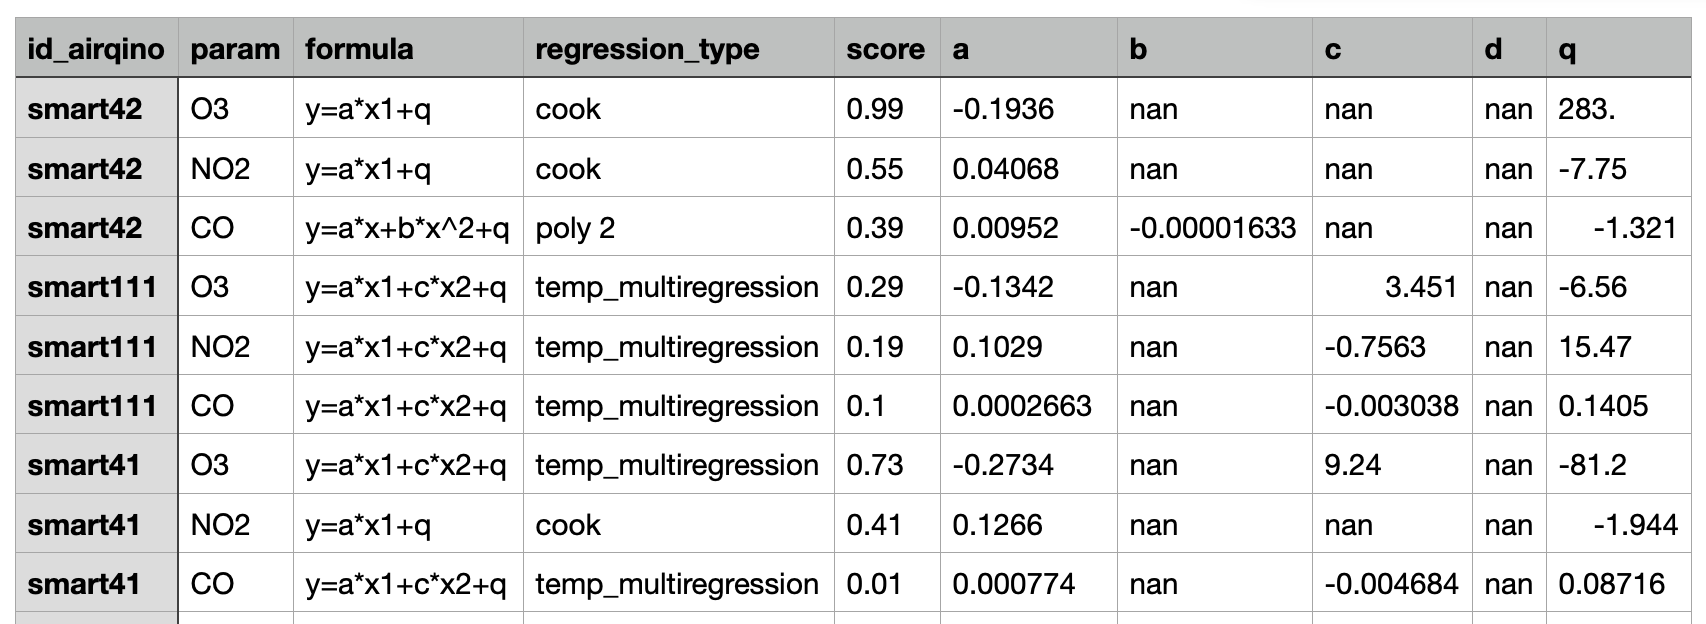
\includegraphics[width=0.75\textwidth,height=\textheight,keepaspectratio]{img/csv_calib}
\caption{Esempio di file csv per calibrazione di centraline AirQino}
\label{fig:csv-calib}
\end{figure}

Dove: 

\begin{itemize}
  \item La colonna \textbf{id\_airqino} indica il nome della centralina AirQino;
  \item La colonna \textbf{param} indica il sensore da calibrare;
  \item Le colonne \textbf{a}, \textbf{b}, \textbf{c} e \textbf{q} rappresentano i coefficienti di calibrazione (rispettivamente \textit{k1}, \textit{k2}, \textit{k3} e \textit{k4} della formula riportata in \ref{sec:motivazioni});
  \item La colonna \textbf{score} indica il coefficiente di determinazione $R^2$;
  \item Le colonne \textbf{formula}, \textbf{regression\_type} e \textbf{d} sono opzionali e riguardano il tipo di regressione e altri parametri al momento inutilizzati (non influiscono sul risultato finale).
\end{itemize}

% Tecnologie utilizzate
\section{Tecnologie utilizzate}\label{sec:tecnologie}

\subsection{Backend}\label{ssec:interfaccia-backend}

\begin{itemize}
  \item \textbf{Flask} \cite{flask} è un framework scritto in Python per la realizzazione di applicazioni web. Ha la caratteristica di essere molto semplice e versatile nella gestione del routing e la creazione di API REST;
  \item \textbf{Pandas} \cite{pandas} è una libreria Python che fornisce strumenti di analisi e manipolazione dei dati. Utilizzata nel progetto per leggere i dati da un file csv;
  \item \textbf{Psycopg2} \cite{psycopg2} è una libreria Python per la connessione a database che utilizzano Postgres (come quello di AirQino);
  \item \textbf{Docker} \cite{docker} è una tecnologia di containerizzazione che consente di organizzare le applicazioni in \textit{container}, componenti isolati che combinano il codice sorgente dell'applicazione con le librerie del sistema operativo e le dipendenze necessarie per eseguire il codice in qualsiasi ambiente. 
\end{itemize}

\clearpage

\subsection{Frontend}\label{ssec:interfaccia-frontend}

\begin{itemize}
  \item \textbf{Angular} \cite{angular} è un framework di applicazioni web, basato su linguaggio TypeScript, che consente la creazione di Single Page Application (SPA) reattive;
  \item \textbf{Bootstrap} \cite{bootstrap} è un framework CSS dedicato allo sviluppo frontend, mettendo a disposizione tipografia, pulsanti, navigazione e altri componenti dell'interfaccia web;
  \item \textbf{ng-bootstrap} \cite{ng-bootstrap} è un set di widget e componenti Angular reattivi che utilizzano lo stile Bootstrap.
\end{itemize}

% Sviluppo
\section{Sviluppo}\label{sec:sviluppo}
Il risultato finale è stato reso disponibile al seguente indirizzo:\

\url{https://airqino-calibration.magentalab.it}.

Di seguito ne vengono descritte le caratteristiche principali.

% Interfaccia
\subsection{Interfaccia}\label{sec:interfaccia}

L'interfaccia, dopo il primo caricamento, si presenta come in figura \ref{fig:interfaccia-1}, con un \textit{form} che permette di scegliere e caricare il file csv, una \textit{checkbox} che consente di aprire una nuova sessione per tutte le centraline, e un pulsante per avviare il caricamento.
\begin{figure}[H]
\centering
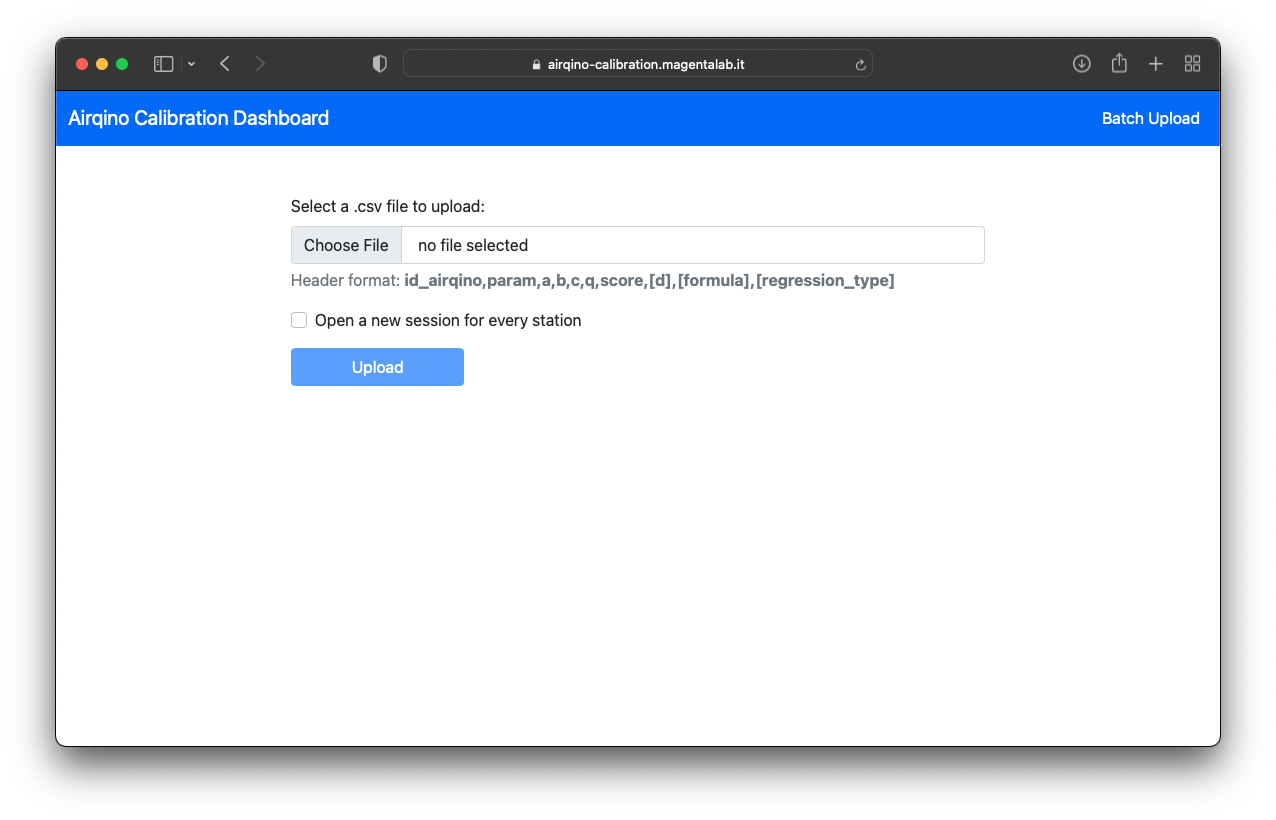
\includegraphics[width=0.70\textwidth,height=\textheight,keepaspectratio]{img/interfaccia_1}
\caption{Interfaccia iniziale dell'applicazione}
\label{fig:interfaccia-1}
\end{figure}

Se il formato del file csv scelto non è compatibile con quello previsto (vedi \ref{sec:requisiti}), la pagina restituisce un errore informativo dove viene indicata esattamente quali colonne mancano nell'header (figura \ref{fig:interfaccia-8}).

\begin{figure}[H]
\centering
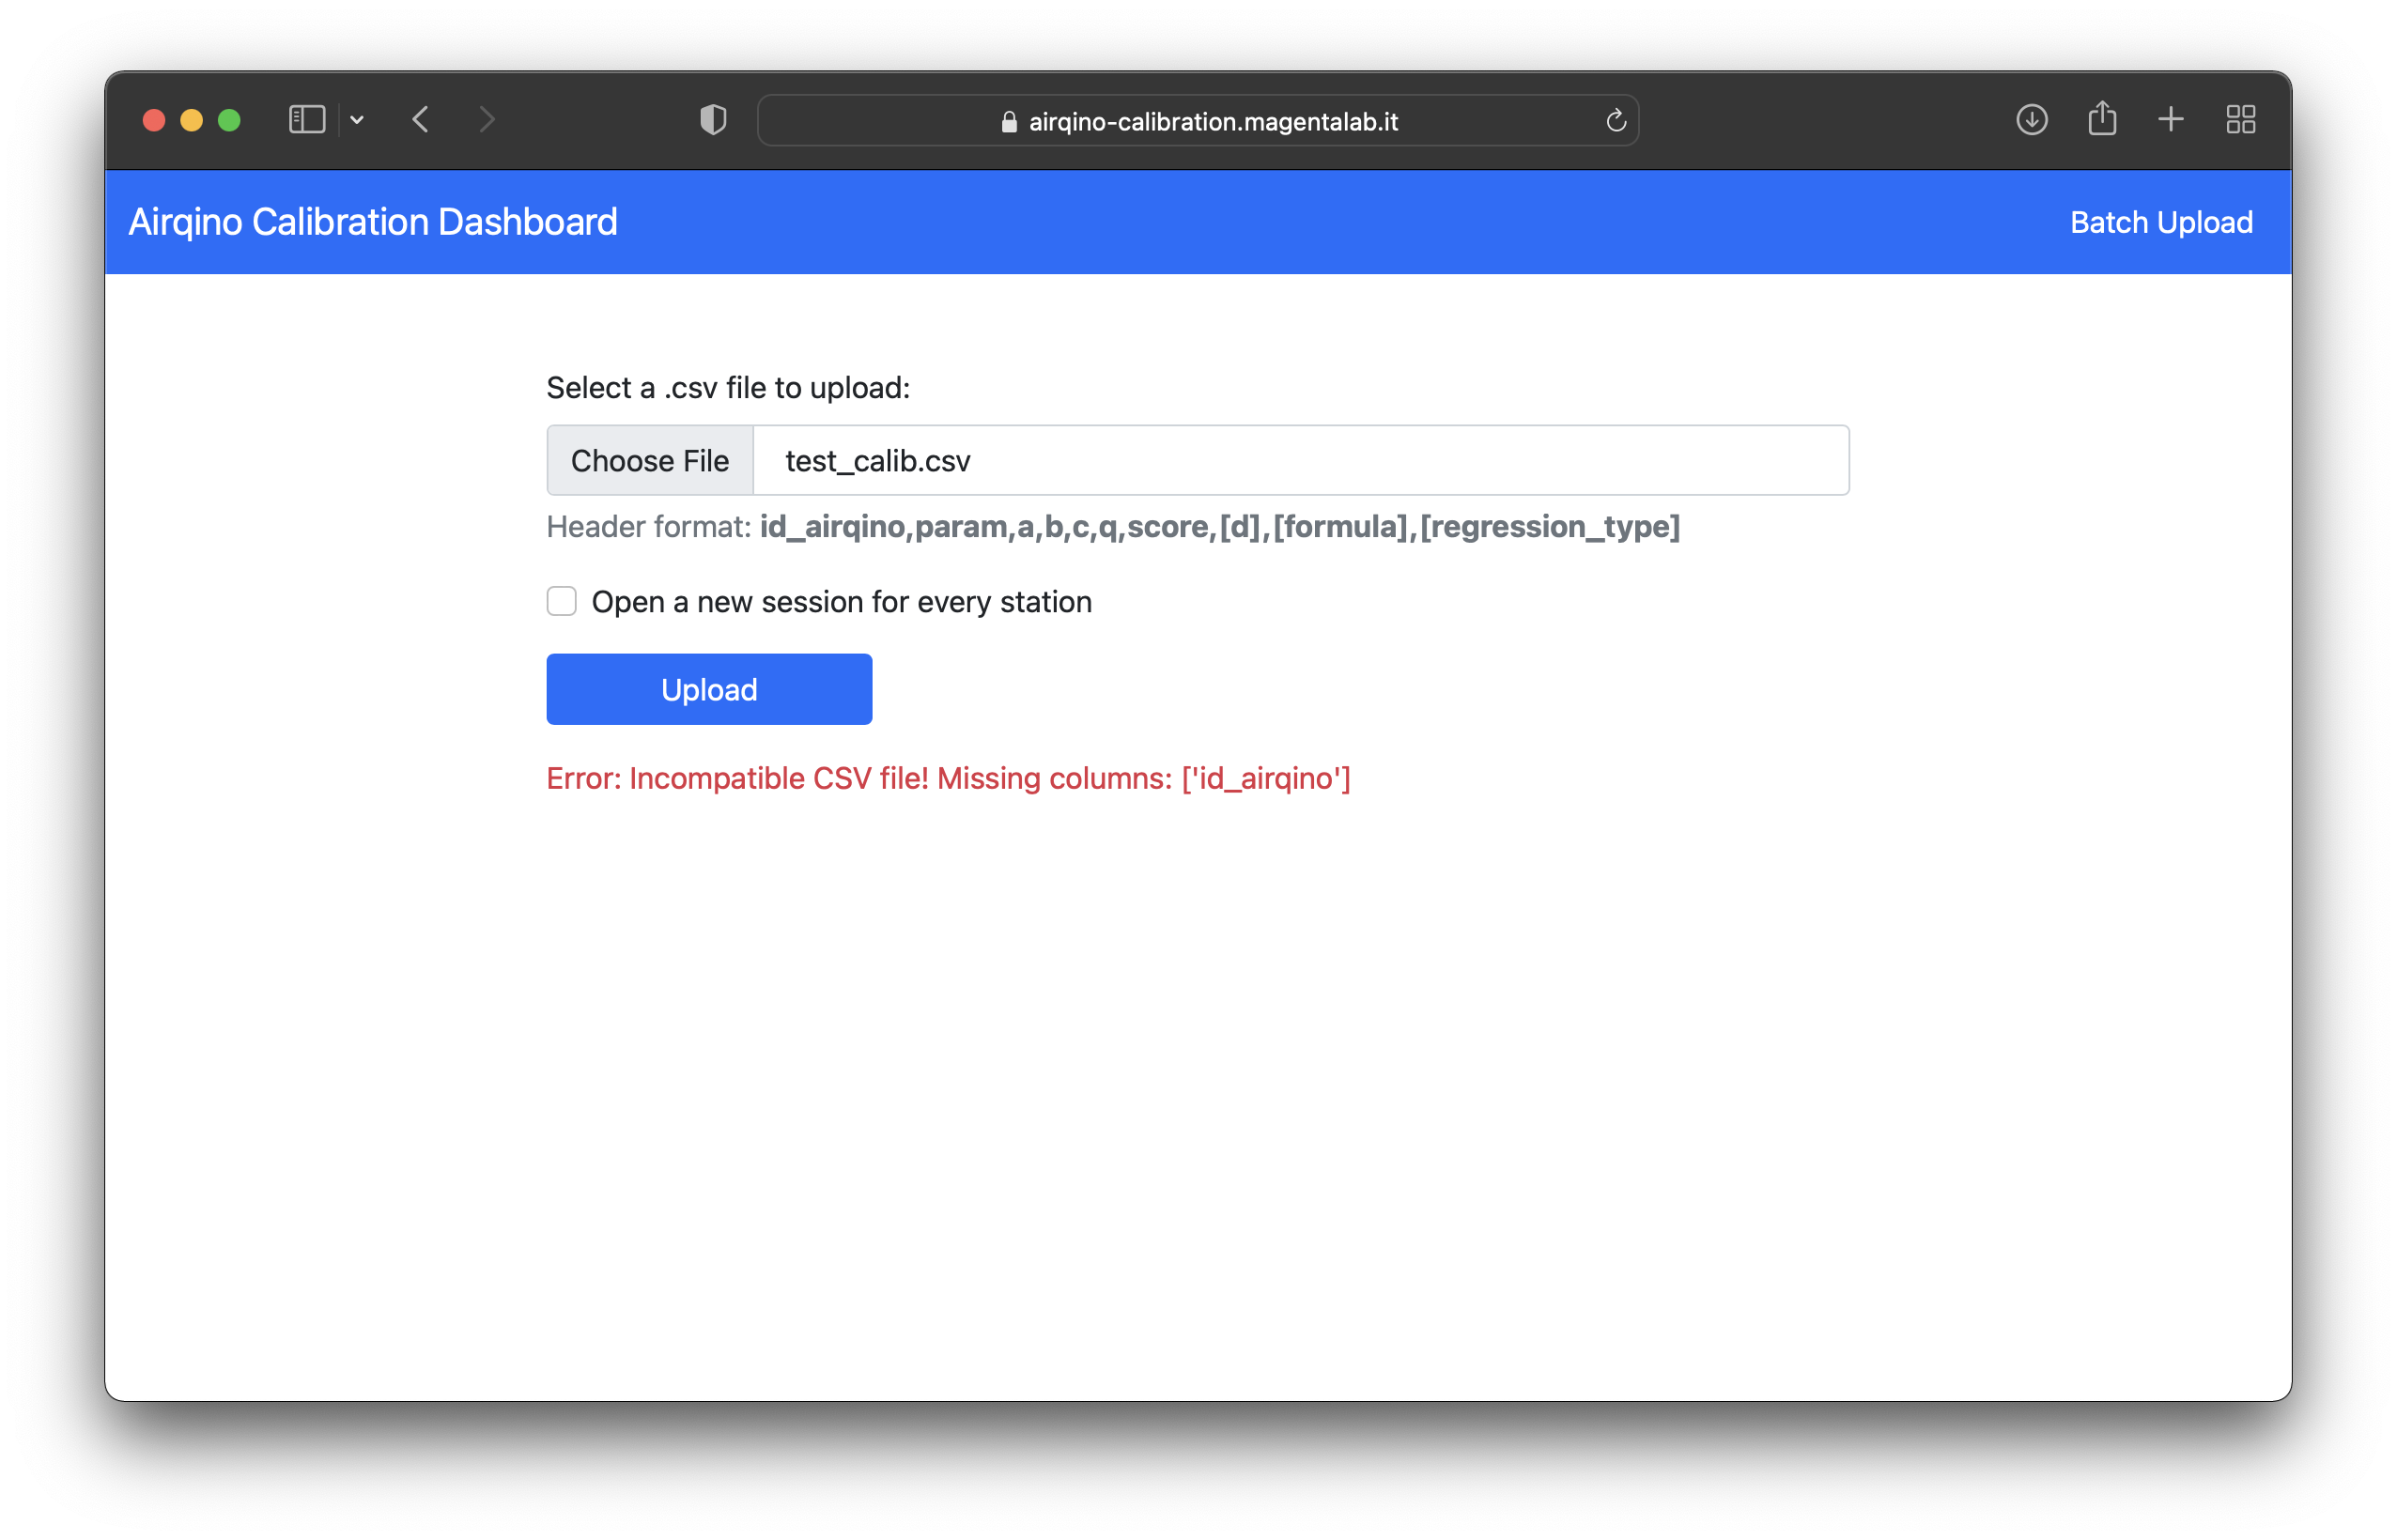
\includegraphics[width=0.70\textwidth,height=\textheight,keepaspectratio]{img/interfaccia_8}
\caption{Errore informativo mostrato in caso di caricamento di un file csv con header non riconosciuto}
\label{fig:interfaccia-8}
\end{figure}

Una pagina simile viene mostrata nel caso in cui l'applicazione non riesca a connettersi al database di AirQino (ad esempio se questo è in fase di mantenimento).

Se il file csv caricato ha il formato corretto, e il database è raggiungibile, viene avviata la procedura di caricamento multiplo dei coefficienti. Al termine dell'operazione, viene mostrato un riepilogo in forma di tabella dove ogni riga corrisponde ad un sensore (figura \ref{fig:interfaccia-2}).

\begin{figure}[H]
\centering
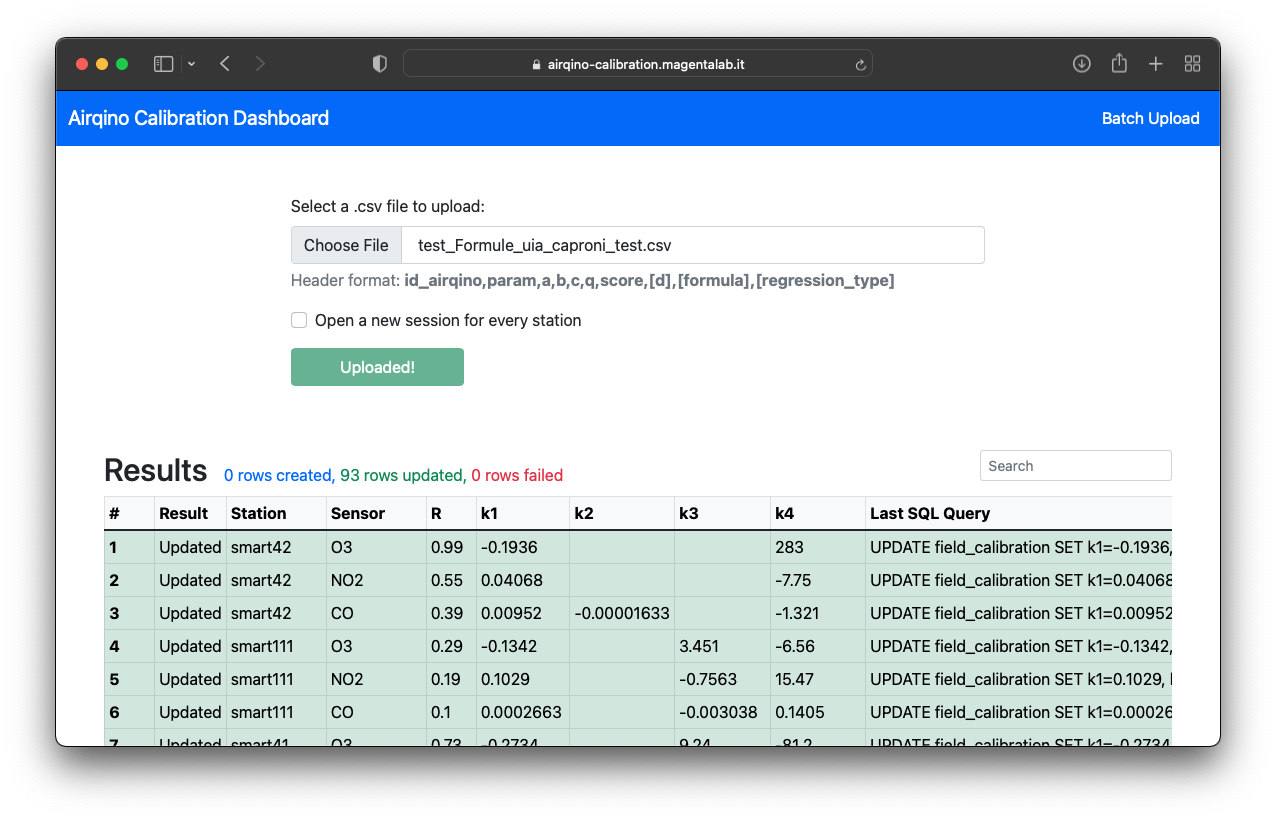
\includegraphics[width=0.70\textwidth,height=\textheight,keepaspectratio]{img/interfaccia_2}
\caption{Interfaccia in caso di caricamento corretto del file csv}
\label{fig:interfaccia-2}
\end{figure}

La tabella, mostrata nel dettaglio in figura \ref{fig:interfaccia-3}, presenta le seguenti colonne:
\begin{itemize}
  \item \textbf{Result}: è l'esito del caricamento sul database (\textit{Updated} se il dato era già presente ed è stato sovrascritto, \textit{Created} se il dato è stato creato per la prima volta, e \textit{Failed} se l'operazione invece è fallita per quel sensore);
  \item \textbf{Station}, \textbf{Sensor}, \textbf{R}, \textbf{k1}, \textbf{k2}, \textbf{k3}, \textbf{k4} sono gli stessi parametri passati nel file csv di input;
  \item \textbf{Last SQL Query}: è l'ultima query effettuata sul database per quel sensore, utile in per verificarne la correttezza e/o capire il motivo di eventuali errori (lo screenshot completo è riportato in figura \ref{fig:interfaccia-6}).
\end{itemize}

\begin{figure}[H]
\centering
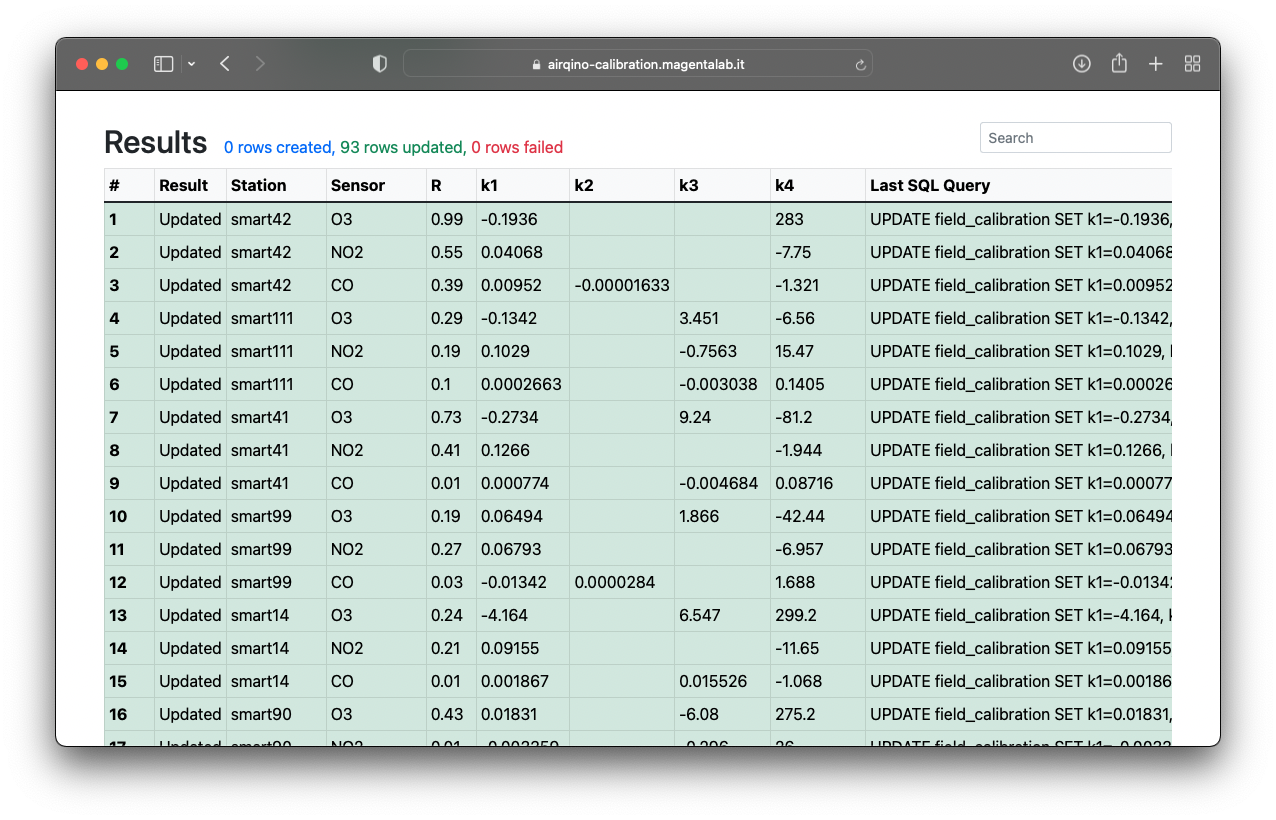
\includegraphics[width=0.70\textwidth,height=\textheight,keepaspectratio]{img/interfaccia_3}
\caption{Dettaglio della tabella di riepilogo del caricamento dei coefficienti}
\label{fig:interfaccia-3}
\end{figure}

\begin{figure}[H]
\centering
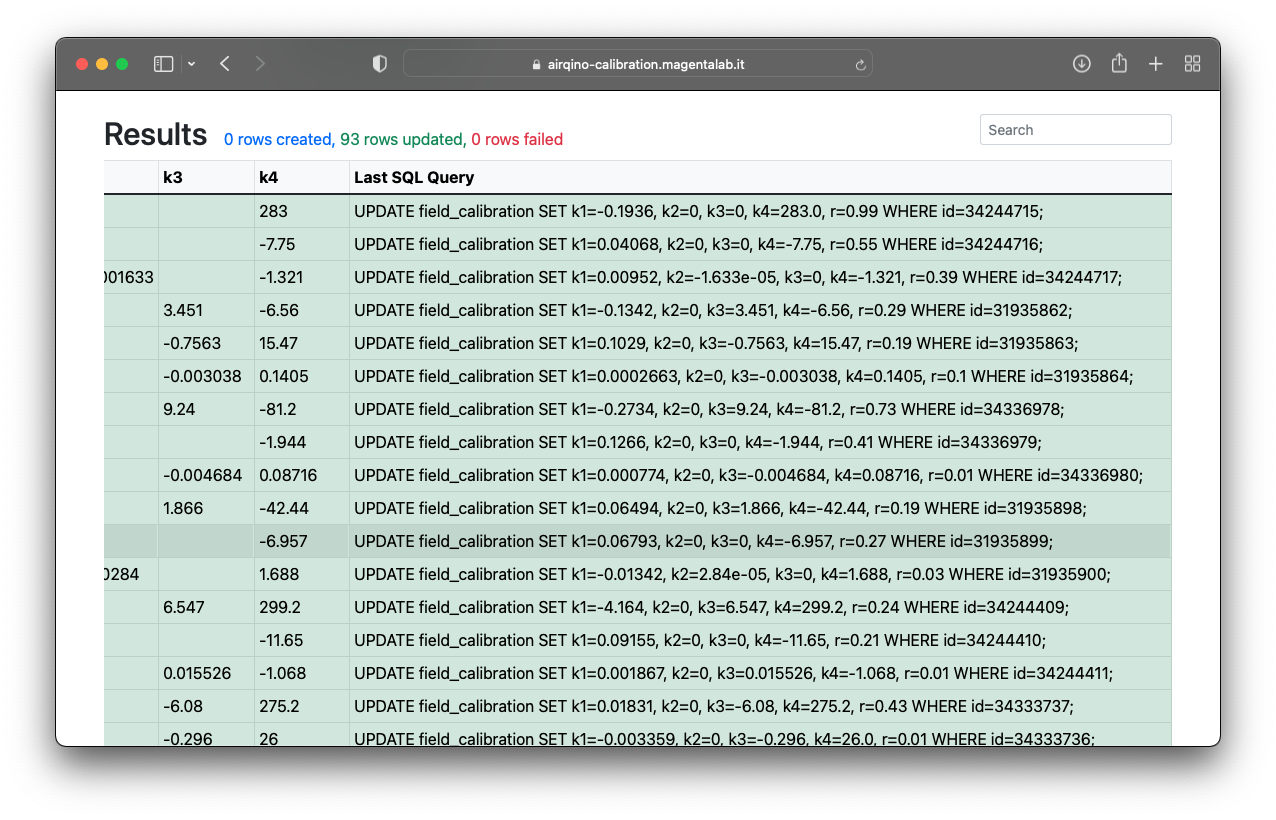
\includegraphics[width=0.70\textwidth,height=\textheight,keepaspectratio]{img/interfaccia_6}
\caption{Dettaglio completo per la colonna \textit{Last SQL Query} della tabella riassuntiva di caricamento dei coefficienti}
\label{fig:interfaccia-6}
\end{figure}

La tabella è ordinabile per colonne (tramite un click su ciascuna di esse) e filtrabile con ricerca \textit{full text} su qualsiasi campo (figura \ref{fig:interfaccia-4-5}).

\begin{figure}[H]%
    \centering
    \captionsetup{justification=centering}
    \subfloat[\centering Ordinamento per colonne]{{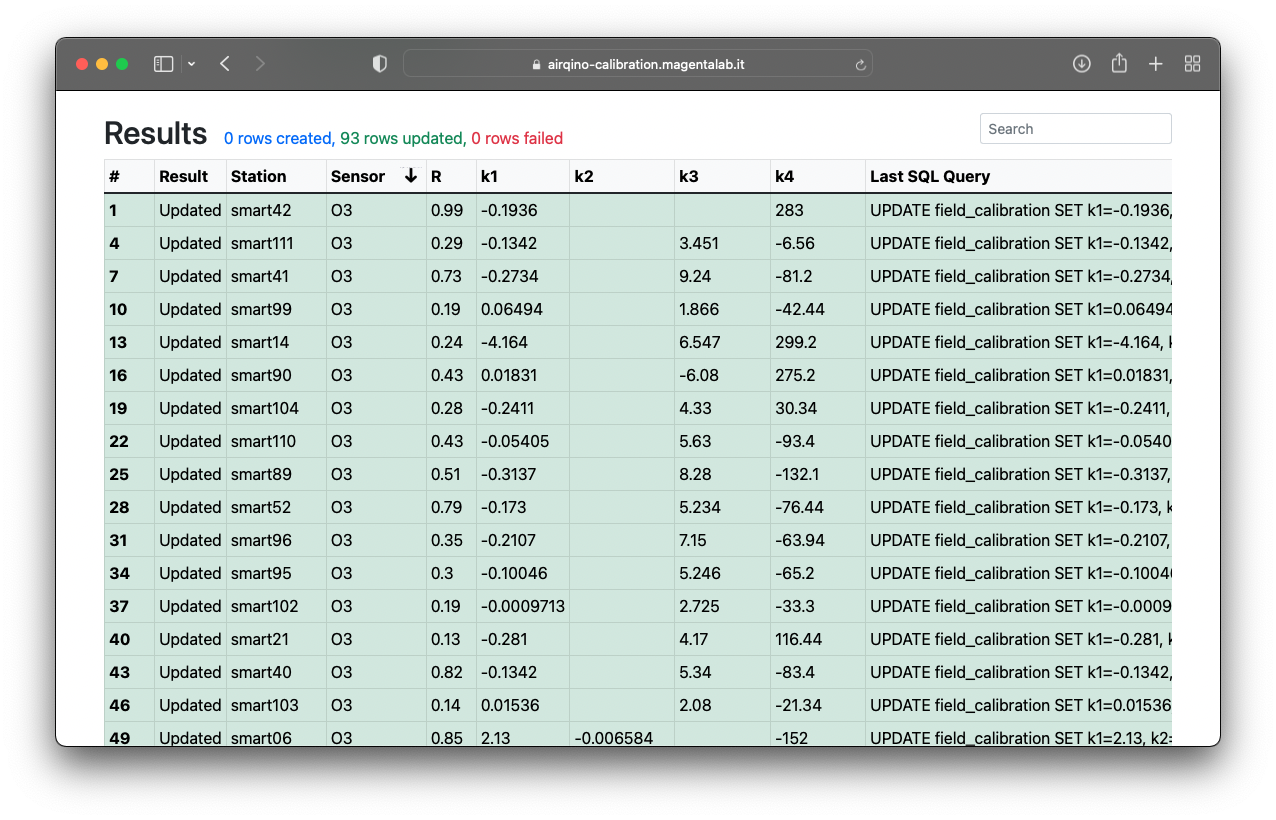
\includegraphics[width=6.9cm]{img/interfaccia_5} }}%
    \subfloat[\centering Filtro con ricerca \textit{full text}]{{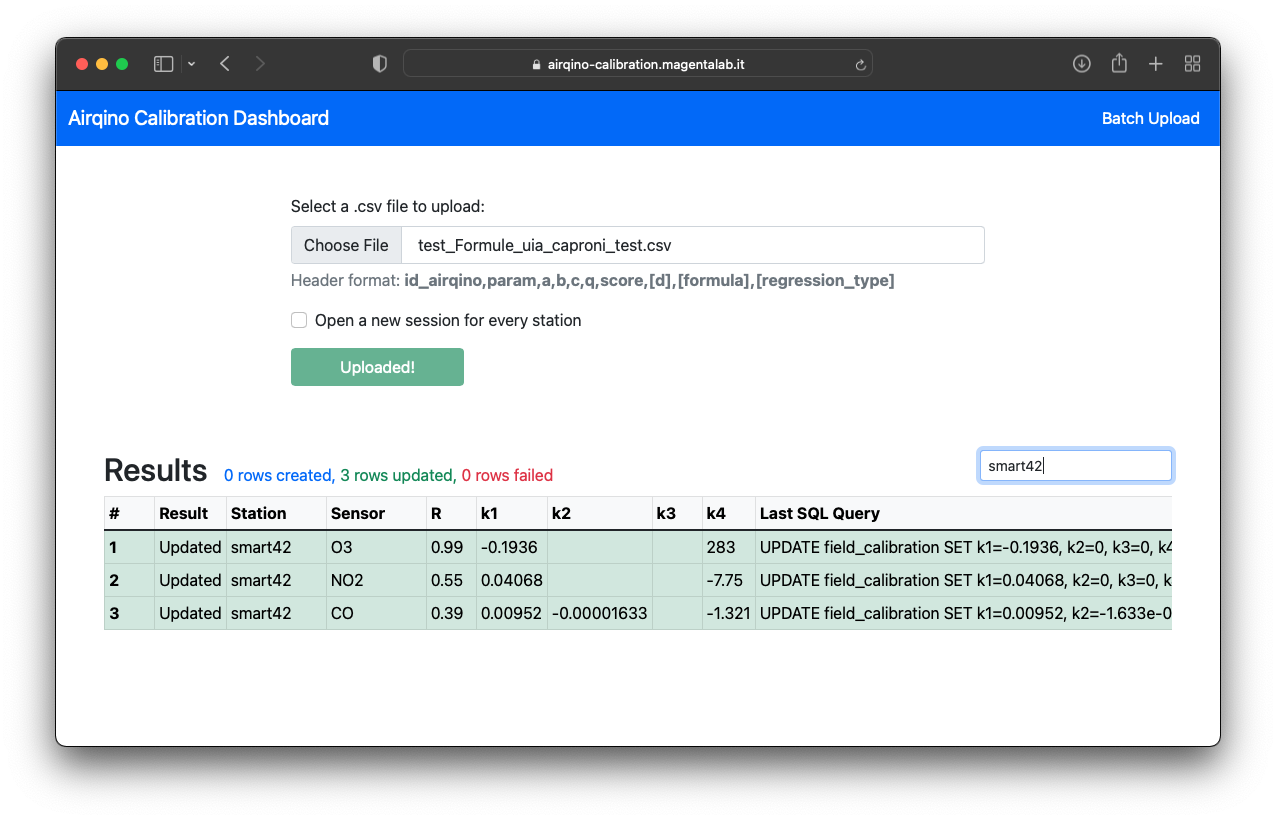
\includegraphics[width=6.9cm]{img/interfaccia_4} }}%
    \caption{Esempio di ordinamento e ricerca della tabella riassuntiva di caricamento dei coefficienti}%
    \label{fig:interfaccia-4-5}%
\end{figure}

In caso di esito negativo per un sensore (ad esempio se il sensore o la centralina specificati non esistono nel database), la riga corrispondente risulta colorata di rosso e la colonna \textbf{Result} fornisce un aiuto nel capire il motivo (es. "Failed: station SMART999 does not exist").
Se invece i coefficienti non erano presenti nel database e sono stati caricati per la prima volta, la riga risulta colorata di azzurro. La figura \ref{fig:interfaccia-7} riporta un esempio di diversa colorazione delle righe in base all'esito: verde per coefficienti aggiornati, rosso per caricamento fallito e azzurro per coefficienti aggiunti per la prima volta.

\vspace{2mm}
\begin{figure}[H]
\centering
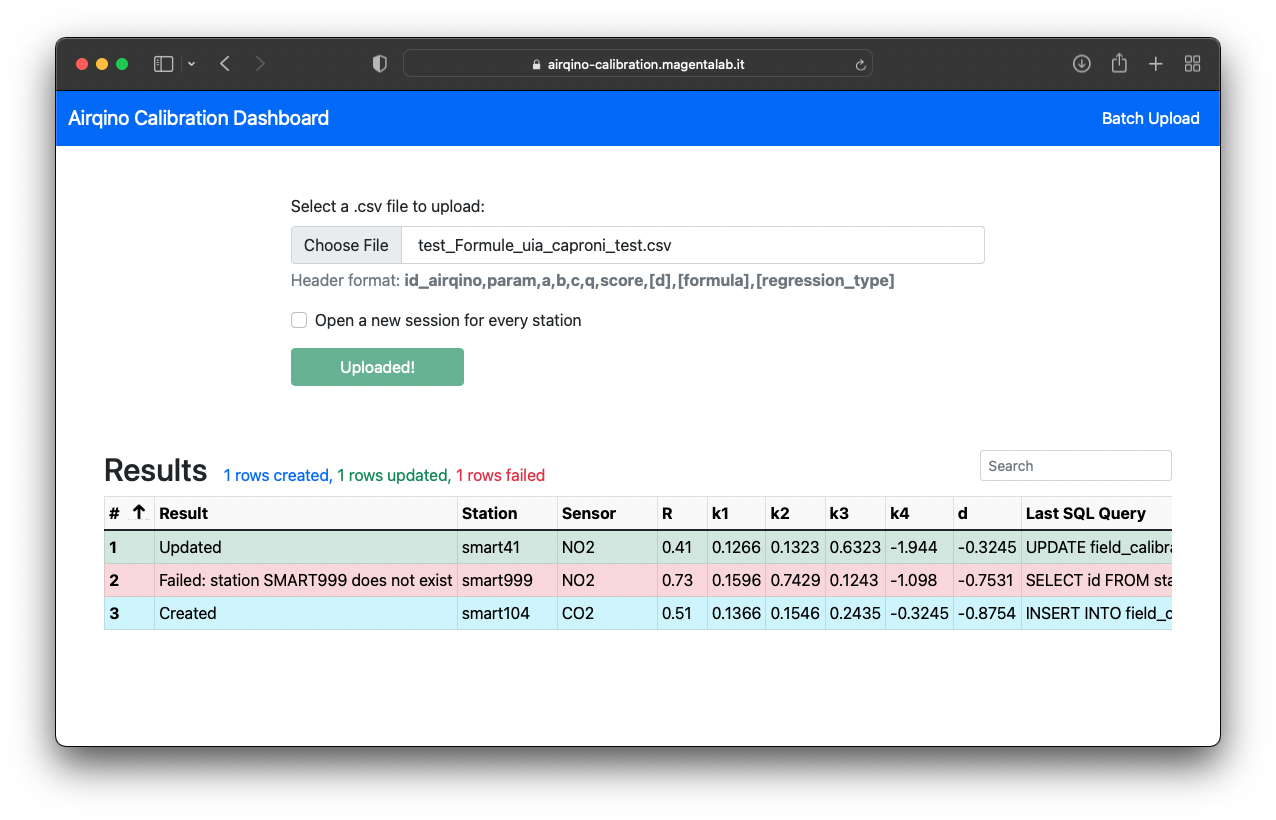
\includegraphics[width=0.60\textwidth,height=\textheight,keepaspectratio]{img/interfaccia_7}
\caption{Esempio di colorazione delle righe della tabella}
\label{fig:interfaccia-7}
\end{figure}

% Autenticazione
\subsection{Autenticazione}\label{sec:autenticazione}
Per la gestione dell'autenticazione è stato scelto il software \textbf{Keycloak} \cite{keycloak}, che risultava essere già installato sul server di Magenta. Keycloak è un prodotto software open source che abilita l'autenticazione \textit{Single Sign-On} (SSO) per applicazioni e servizi. È scritto in Java e supporta i protocolli di federazione delle identità per impostazione predefinita SAML v2 e OpenID Connect (OIDC) o OAuth2. \cite{keycloak}

In particolare, Keycloak consente a un'applicazione di delegare la propria autenticazione ad un server web predisposto, consentendo allo sviluppatore di concentrarsi sulle funzionalità, senza doversi preoccupare di aspetti di sicurezza e crittografia. Keycloak infatti include un server e un agente: l'agente è installato sulle applicazioni che richiedono l'autenticazione, mentre il server gestisce tutte le richieste di autenticazione. Quando un utente tenta di accedere a una applicazione protetta da Keycloak, l'agente verifica se l'utente è autenticato e, in caso affermativo, fornisce le credenziali appropriate all'applicazione.

\begin{figure}[H]
\centering
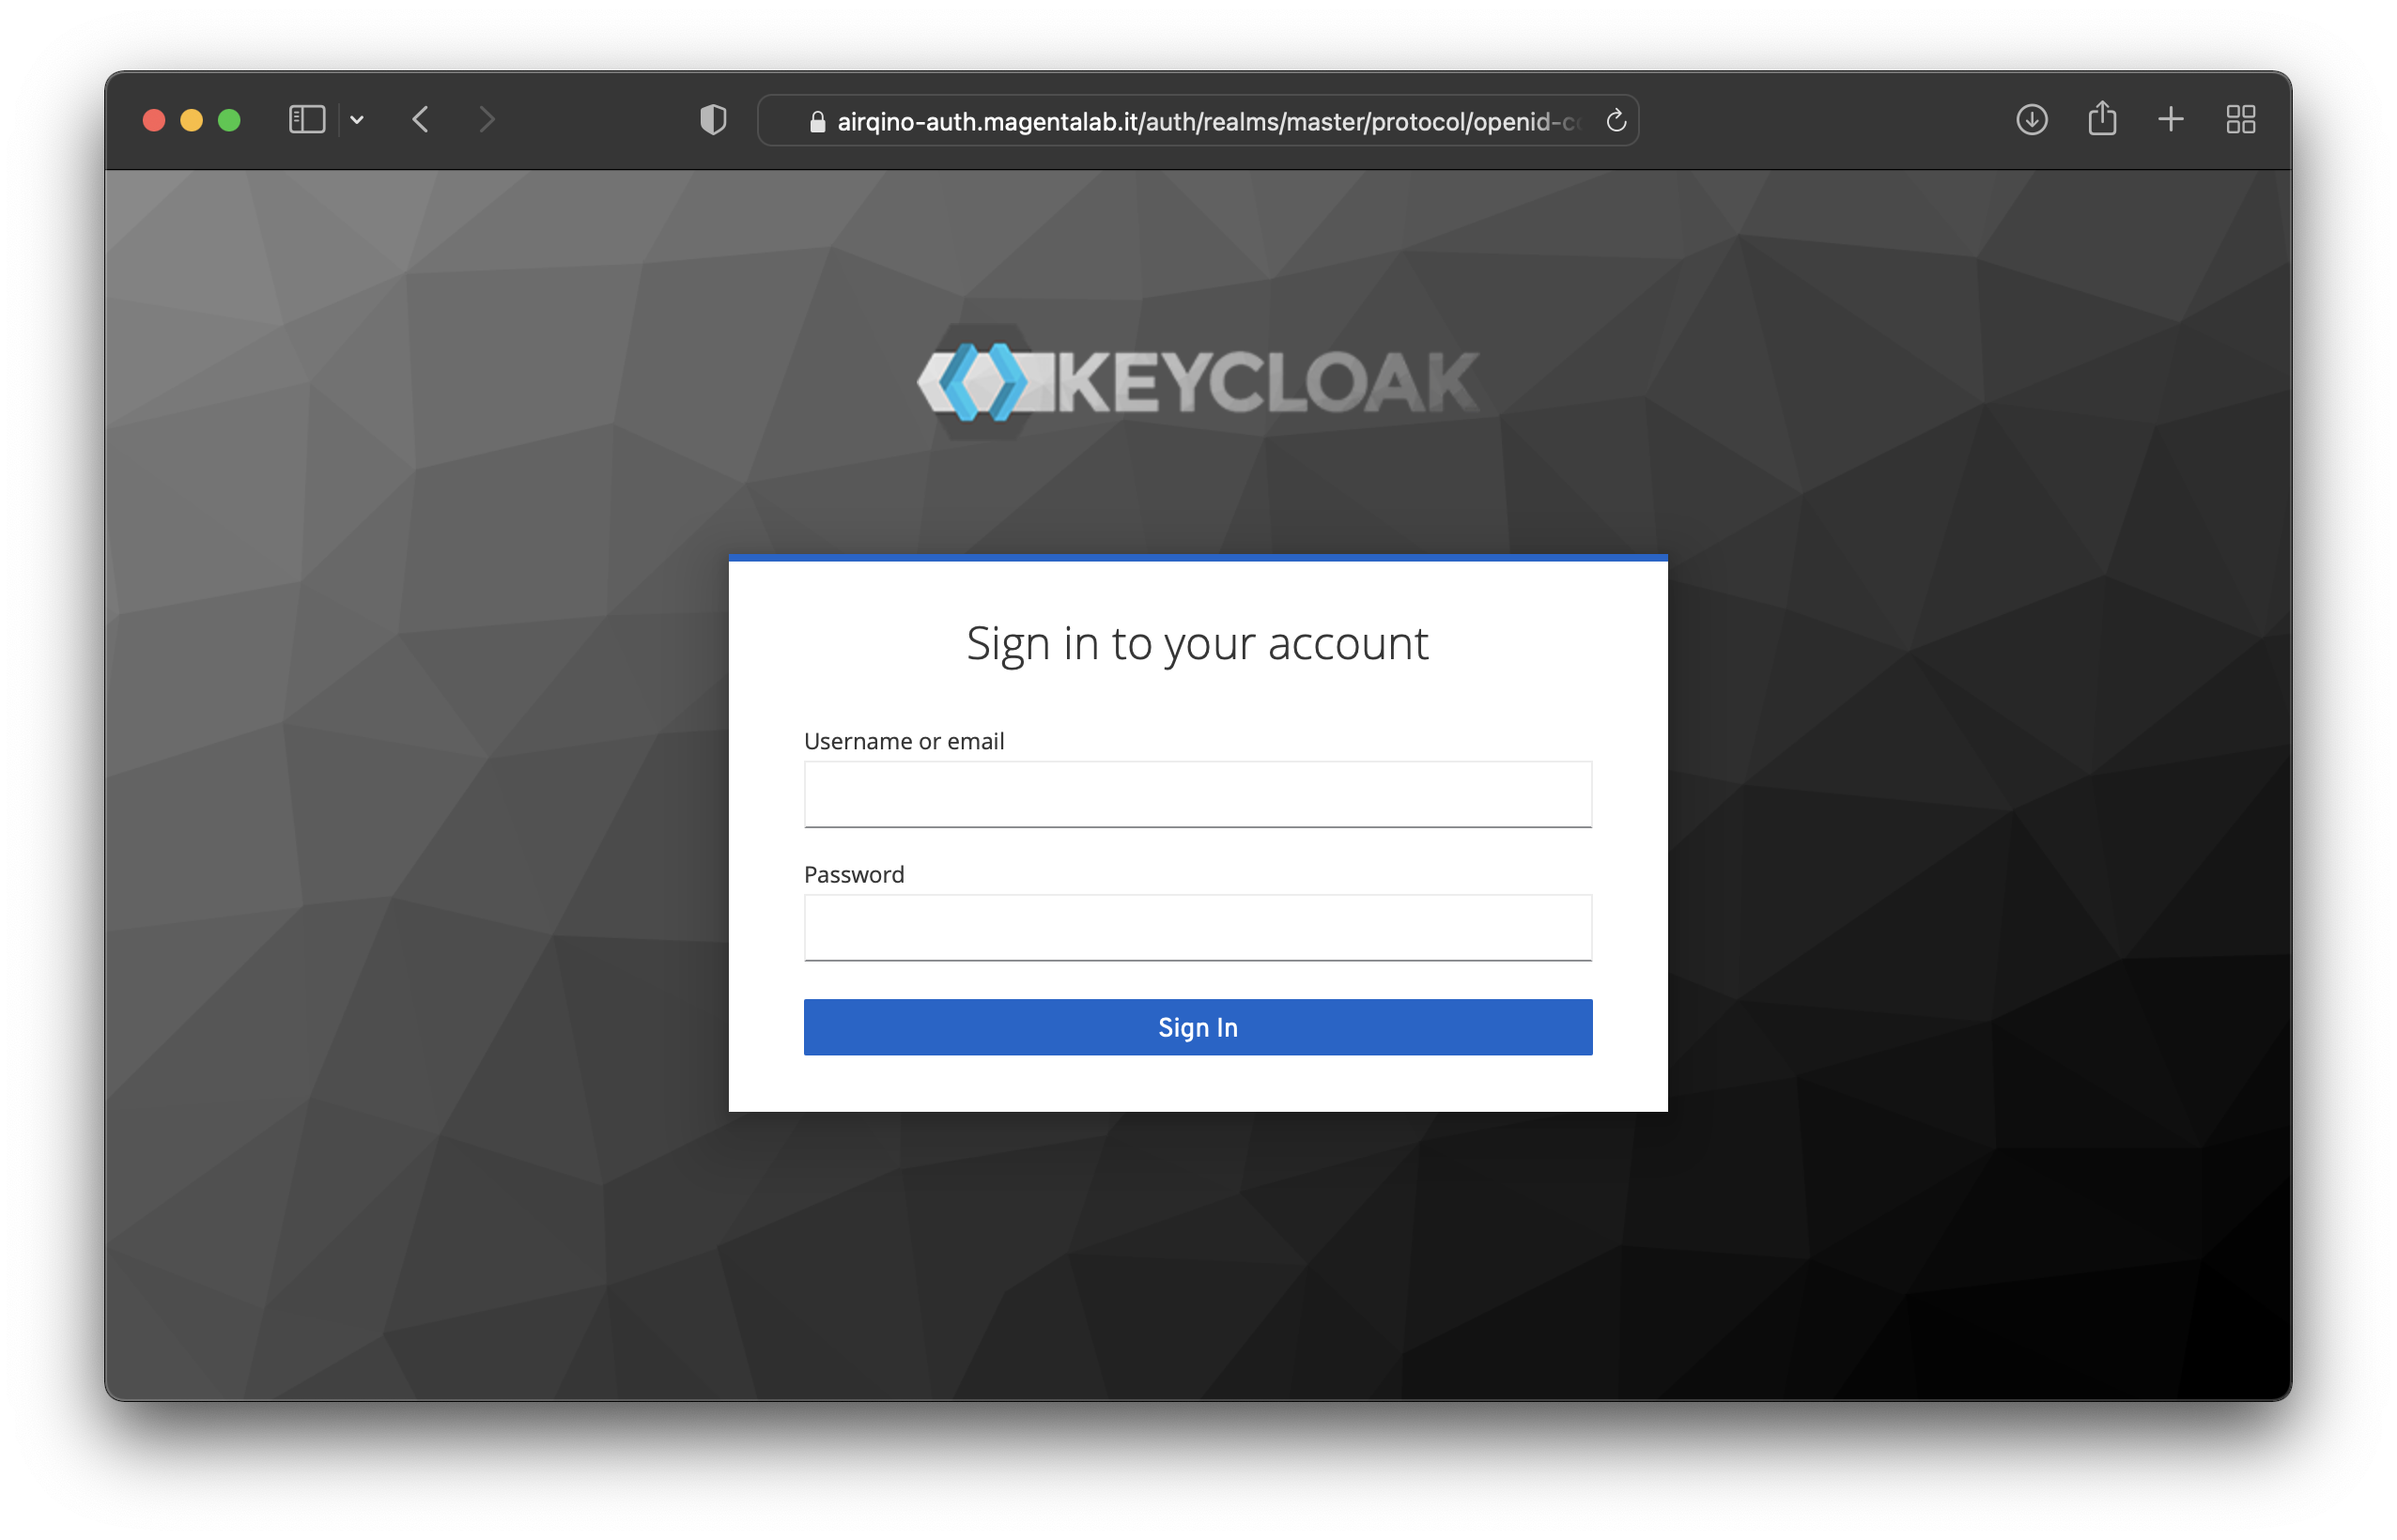
\includegraphics[width=0.70\textwidth,height=\textheight,keepaspectratio]{img/keycloak}
\caption{Autenticazione con Keycloak}
\label{fig:keycloak}
\end{figure}

Keycloak è stato integrato nell'applicazione con l'aiuto della libreria open source \url{keycloak-angular} \cite{keycloak-angular}, un wrapper della libreria ufficiale JavaScript \url{keycloak-js} \cite{keycloak-js} che rende semplice l'utilizzo del software per applicazioni Angular. I principali parametri da impostare sono:

\begin{itemize}
  \item \textbf{url}: l'url del server Keycloak;
  \item \textbf{realm}: il nome del \textit{realm}, impostato nel pannello di amministrazione, che serve a gestire un insieme di utenti, credenziali e ruoli;
  \item \textbf{clientId}: l'identificativo del \textit{client}, cioè l'entità che richiede a Keycloak il permesso di autenticare un utente, anche questo impostato nel pannello di amministrazione;
  \item \textbf{initOptions}: le opzioni di configurazione, ad esempio è possibile specificare se l'autenticazione avviene automaticamente al caricamento della pagina (come in questo caso) oppure scatta in un secondo momento (utile se ad esempio l'applicazione fornisce funzionalità anche senza loggare l'utente).
\end{itemize}

È possibile inizializzare la configurazione in un file JavaScript di questo tipo (file \url{keycloak-init.js}, da caricare poi all'avvio del modulo principale dell'applicazione):

\vspace{1mm}
\begin{lstlisting}[language=js]
import {KeycloakService} from "keycloak-angular";

export function initializeKeycloak(keycloak: KeycloakService) {
  return () =>
    keycloak.init({
      config: {
        url: 'https://airqino-auth.magentalab.it/auth',
        realm: 'master',
        clientId: 'calibration',
      },
      initOptions: {
        onLoad: 'login-required',
        flow: 'implicit'
      },
    });
}
\end{lstlisting}

Questi parametri sono sufficienti a definire l'integrazione tra applicazione e server Keycloak, garantendo in maniera efficiente funzionalità di autenticazione e autorizzazione.

% CI/CD e deploy automatico
\subsection{CI/CD e deploy automatico}\label{sec:ci}
L'integrazione continua (\textit{continuous integration}, CI o CI/CD) è una metodologia di sviluppo software \textit{agile}, spesso utilizzata in combinazione con approccio \textbf{DevOps}, che prevede la continua e costante integrazione dei cambiamenti effettuati dagli sviluppatori all'interno di un codice sorgente (figura \ref{fig:cicd}).

Con il termine CD (\textit{continuous delivery}) si indica invece la distribuzione e/o il deployment continuo, un concetto comunque correlato alla CI, ovvero processo con il quale le modifiche apportate da uno sviluppatore all'applicazione vengono automaticamente testate e caricate in una repository, dalla quale vengono automaticamente distribuite in un ambiente di produzione. \cite{cicd}

\begin{figure}[H]
\centering
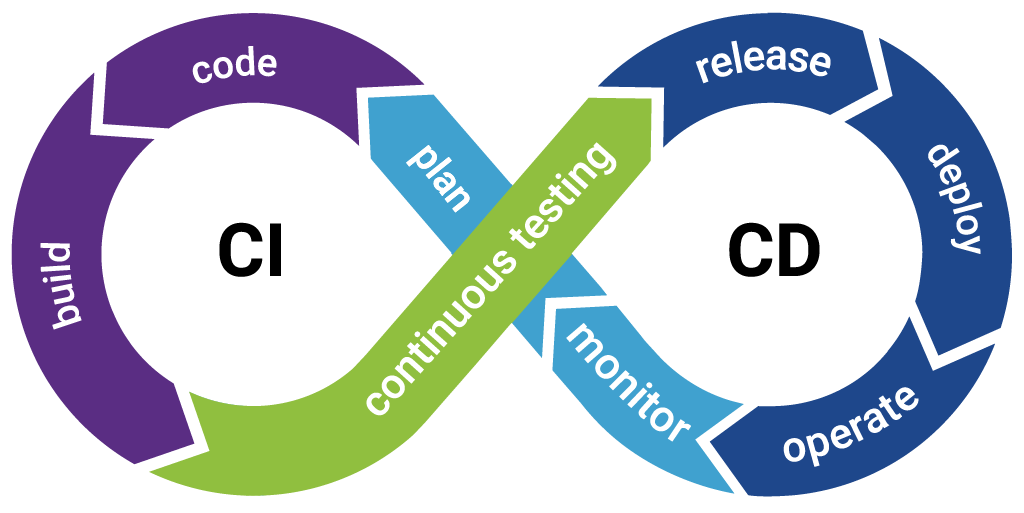
\includegraphics[width=0.65\textwidth,height=\textheight,keepaspectratio]{img/ci}
\caption{Schema di funzionamento CI/CD\\Fonte: \url{flagship.io}}
\label{fig:cicd}
\end{figure}

La CI/CD porta diversi vantaggi, tra cui:
\begin{itemize}
  \item Solidità del prodotto, poiché le integrazioni sono frequenti e anche i test vengono eseguiti in anticipo;
  \item Aumento della qualità del codice;
  \item Consegna più rapida del software.
\end{itemize}

Lo strumento di CI scelto per questa applicazione è \textbf{Jenkins} \cite{jenkins}. Si tratta di un software open source di integrazione continua, scritto in Java, che permette di automatizzare il processo di integrazione dei cambiamenti all'interno di un codice sorgente, con la possibiltà di eseguire una serie di controlli per verificarne la correttezza.\\

Tra le varie caratteristiche, Jenkins offre un sistema chiamato \textit{pipeline}, ovvero uno script (chiamato \textit{Jenkinsfile}) che fornisce a Jenkins una serie di lavori (\textit{stage}) da eseguire in modo simile a una pipeline (uno dopo l'altro).

Il \url{Jenkinsfile} utilizzato per questo progetto contiene tre stage, ognuno con i propri comandi, ed è riportato di seguito (ridotto per semplicità):

\vspace{1mm}
\begin{lstlisting}[]
pipeline {
    agent any
    stages {
		stage('Build Angular frontend') {
			steps {
			    sh 'npm install && ng build --configuration production'
			}
		}
		stage('Docker deploy backend') {
			steps {
				sh 'flask run'
			}
		}
		stage('Deploy frontend') {
			steps {
			    'scp -r dist/* ${HOST}:${PATH}/'
			}
		}
    }
}
\end{lstlisting}

In particolare:

\begin{itemize}
  \item Il primo stage esegue il build del frontend, installando le dipendenze con \url{npm} \url{install} e avviando il processo con \url{ng} \url{build} in configurazione di produzione. Questo genera l'artefatto finale all'interno della cartella \url{dist};
  \item Il secondo stage esegue il rilascio del backend con il comando \url{flask} \url{run};
  \item Infine, il terzo stage rilascia il frontend copiando i contenuti della cartella \url{dist} nella cartella corretta del server di produzione.
\end{itemize}

L'interfaccia web di Jenkins permette inoltre di monitorare l'andamento dei vari step e di verificare eventuali errori. Jenkins può essere anche combinato con Docker \cite{docker} in modo da garantire processi di rilascio automatizzati e allo stesso tempo avere l'isolamento delle dipendenze, che verranno installate solo sul container e non su tutto il server.

